\section{Redegørsel for Mindste Kvadraters Metode}\label{sec:redegorsel}
Antag at du har en række data. Disse data beskriver en sammenhæng mellem tid og distance for en bil. Bilen kører med en konstant hastighed. Du har nu brug for at finde ud af hvor langt bilen har kørt efter 10 sekunder. Dette ingår dog ikke i datasættet. For at finde denne information kunne man fx. opstille en funktion der beskriver denne sammenhæng. For at beskrive denne sammenhæng, kunne Mindste Kvadraters Metode anvendes. Mindste Kvadraters Metode anvendes ofte til at beskrive en ret linje. (\begin{math}y = ax + b\end{math}) En ret linje kan beskrives på mange måder. Dog vil der kun være en linje der beskriver datasætte bedst. For at finde frem til det krever det, at der fordybes i funktioner af to variable, samt hvordan de afledes.

% Redegør for matematikken bag Mindste Kvadraters Metode (Få sammen sat afsnitet funktioner med to variable og Mindste Kvadraters Metode på en god måde)

\subsection{Funktioner med to variable?}\label{sec:FunktionerMedToVariable}
Du har måske stiftet bekendtskab med funktioner af én variabel. Disse funktioner skrives ofte som $f(x) = x^2$, hvor man indsætter en værdi for $x$ og beregner den tilsvarende værdi af $f(x)$. Her giver man altså en værdi og får en værdi tilbage. Men hvad nu hvis du skal beskrive en sammmenhæng, der er afhængig af to variabler? Her kommer funktioner med to variabler ind i billedet. Når der arbejdes med funktioner af en variabel vil den grafiske afblidning forgå i et koordinatsystem med en x-akse og en y-akse. Altså et todimensionelt koordinatsystem. For at kunne afbillede funktioner af to variable, arbejdes der ikke længere i et koordinatsystem, med todimensioner, men i et tredimensionelt koordinatsystem. Her er der en x-akse, en y-akse og en z-akse. Den nye akse (z-aksen) står vinkelret på de to andre akser (\cite[246-248]{funktionrAfToVariable}). For at bedre forstå, hvordan det tredimensionelle koordinatsystem hænger sammen, kan man tænke på det som en kasse, hvor  $x-aksen$ er længden, $y$-aksen er bredden, og $z-aksen$ er højden. Når der arbejdes med funktioner af to variable, vil den typiske notation se således ud: $f(x,y)$. Her er både $x$ og $y$ variable. Disse to variable kan bruges til at beskrive et punkt i det tredimensionelle koordinatsystem. Dette skyldes, at $z = f(x,y)$. Et eksempel kunne være et vejrkort, hvor temperaturen ($z$) afhænger af geografiske koordinater ($x, y$). Her angiver $x$ og $y$ en lokation, og $z$ angiver temperaturen ved dette punkt. På den måde afhænger temperaturen af to variable, nemlig det geografiske punkt, som beskrives ved $(x, y)$. \\
I forbindelse med Mindste Kvadraters Metode bruges funktioner af to variable til at beskrive summen af kvadraternes areal mellem punkt og en linje. I denne sammenhæng opstilles funktionen $f(a, b)$, hvor $a$ og $b$ er de parametre, der bestemmer linjens hældning og skæring. Denne funktion kan opfattes som en flade i et tredimensionelt koordinatsystem. 
For at finde den linje, der bedst passer til datasættet, skal værdierne af $a$ og $b$ findes. Dette kræver, at der arbejdes med metoder til at finde minimumspunkter i funktioner af to variable. Grunden til hvorfor minimumspunktet skal findes forklares i afsnit \ref{sec:bedsteFunktion}. Hvordan minimumspunktet findes forklares dog i næste afsnit.
% Hvad mangler der at blive redegjort for i dette afsnit? Grafisk afblidning af funktion. Saddelpunkt?)


\subsubsection{Partielt differentiation}\label{sec:PartieltDifferentiation}
For at finde hældningen af tangenten til en funktion af to variable, skal man gå igennem en lidt længere proces end ved funktioner af en variabel. For at finde hældningen af tangenten til funktionen af en variabel, diffrencere man med hensyn til $x$. Et eksempel kunne være $f(x) = x^2$ her er $f'(x) = 2x$. Dette skyldes følgende regneregl: $a \cdot x^n$ bliver til $a \cdot n \cdot x^{n-1}$. \\ Ved funktioner af to variable krærver dette at man benytte sig af en metode kaldt: \textit{Partial differentiation}. Ved partial differentiation, tages der fat i en variabel ad gangen. Partial betyder delvis. Grunden til at dette ord anvendes er da man diffrencere mht. $x$ og $y$ i hver deres led (\cite[4]{Larsen2016}). Her undersøges, hvordan funktionen ændrer sig med hensyn til en variabel, mens den anden betragtes som konstant. Opgaven er nu at finde den partial aflededet funktionen. For at finde den partielle afledede for funktionen $f(x,y)$ startes der med at sætte en af variablerne til en konstant. I dette tilfælde sættes $y$ til en konstant. Når der diffrenceres med en funktion af en variabel, agives dette sådan: \begin{equation}\frac{d f(x)}{d x}\end{equation} Sådan er det dog ikke ved partial differentiation. Her angives det sådan: \begin{equation}\frac{\partial f(x,y)}{\partial x}\end{equation} 
Det bløde $d$ ($partial$) angiver at der differentieres partielt. For at illustrere dette kan funktionen $f(x,y) = x^2 + 3y^2$ tages som eksempel. Målet er at finde de partielle afledede af $f(x,y)$. Først diffrenceres der med hensyn til $x$, mens $y$ dermed betragtes som en konstant. Regnereglerne forskriver at en konstant bliver til nul når den diffrenceres. Dernest anvendes regnereglen, der forskriver at \begin{math}a \cdot x^n\end{math} bliver til \begin{math}a \cdot n \cdot x^{n-1}\end{math} \cite[14]{Pihl2019}. Dermed må den partial aflededet mht. x være: 
\begin{equation}\frac{\partial f(x,y)}{\partial x} = 2x\end{equation}
På samme måde findes den partielle afledede med hensyn til $y$ ved at betragte $x$ som konstant. Dette giver:
\begin{equation}\frac{\partial f(x,y)}{\partial y} = 6y\end{equation}
Ved Mindste Kvadraters Metode anvendes denne teknik til at finde ekstremumspunkter for funktioner af to variable. Ekstremumspunkterne repræsenterer de værdier for parametrene $a$ og $b$, der minimerer summen af kvadrerede afvigelser mellem datapunkterne og modellen. Dette uddybes i det følgende afsnit.
\newpage
\subsection{Sådan finder du frem til den bedste funktion}\label{sec:bedsteFunktion}
I de foregående afsnit er der blevet redegjort for funktioner af to variable og, hvordan de differentieres. Der er også blevet forklaret, hvorfor disse metoder er relevante, og hvordan de kan bruges i forbindelse med Mindste Kvadraters Metode. For at finde den bedste funktion skal der først udvikles en metode til at beskrive, hvor godt en funktion passer til et datasættet. Den nemmeste måde at beskrive hvor godt en linje passer på et datasæt vil nok være at beskrive afstanden fra punkt til linje. Dette kan gøres på flere måder. Afstanden kunne være den vinkelrette afstand fra linjen ned til punktet. dette er dog ret svært at regne med. I stedet for det kan den lodrette afstand fra punkt til linje findes. Dette gøres ved at finde forskellen i y-værdierne.
\begin{wrapfigure}{r}{0.5\textwidth}
    \centering
    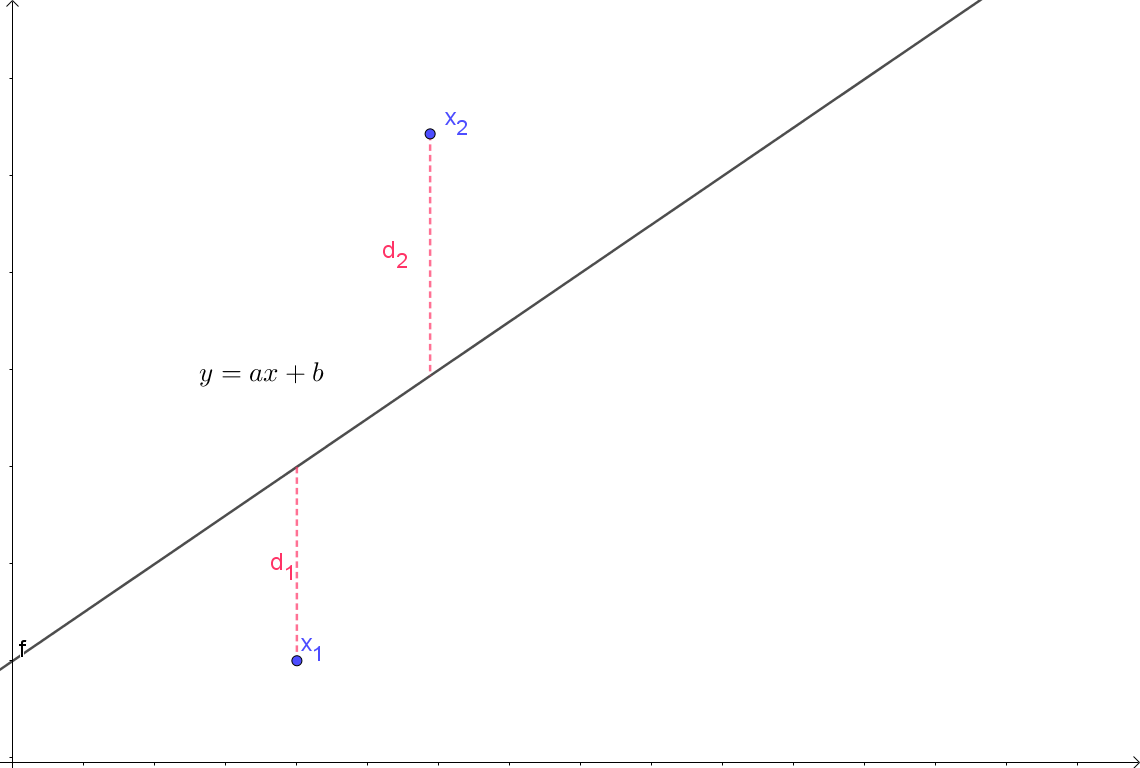
\includegraphics[width=0.5\textwidth]{figures/afstand.png}
    \caption{Afstand fra punkt til linje}
    \label{fig:afstandFraLinjeTilPunkt}
\end{wrapfigure}   
Dette skaber dog en udfordring som man skal være opmærksom på. Nemlig at der kan være punkter over og under linjen. En distance kan altså derfor både være positiv og negativ. For at undgå at dette bliver et problem opløftes afstanden i anden. (\cite[2]{ForberedelsessetMaj2013}). Se figur \ref{fig:afstandFraLinjeTilPunkt} for grafisk ilustration \\ Da der nu er styr på hvordan afstanden fra punkt til linje findes. Skal der nu findes en metode hvorpå det er muligt at beskrive afstanden ift linjen. Hvis der startes med at tage udgangspunkt i et punkt. Punktet kunne hede hvad somhelst. Linjen hedder dog altid: $y = a \cdot x + b$. Så må afstanden i y-værdien kunne beskrives som:  
\begin{equation}\label{eq:distance}
    d_n = a \cdot x_n + b - y_n
\end{equation} grunden til at $y_n$ fratrækkes, er at y-værdien for linjen ved $x_n$ ville være $y = a \cdot x + b$. Isoleret set så er afstanden y-værdien for funktionen minus y-værdien for punktet. På den måde kan afstanden altså bestemmes. Afstanden har på den måde nu dannet en ligning med to ubekendt. Til sammen beskriver de arealet af en kvadrat. Grunden til at de beskriver arealet af en kvadrat er da afstanden som nævnt før opløftes i anden. Det må derfor være det samme som at regne arealet af en kvadrat (\cite{Bentzen2014}). Nu begynder navnte Mindste Kvadraters Metode lige så stille at give mening. Da målet er at finde den linje hvor Kvadraternes areal er mindst. For at regne distance fra alle punkter til linjne anvendes den formlen som blev introduceret før (Formel: \ref{eq:distance}). Deres fælles areal kan derfor beskrives som følgende:
\begin{equation}\label{eq:formularForDistanceForAllDataPoints}A = \sum_{n=1}^n (a \cdot x_n + b - y_n)^2\end{equation}
Resultat af denne udregning kunne omskrives til en funktion af to variable, hvor $a$ og $b$ er de ubekendte. Der hvor arealerne er mindst må de to ubekendte danne den best mulige linje. Dette ville kunne ses som et ekstrema, på funktionen af variablerne $a$ og $b$. Dette ekstrema findes ved at lave partial diffrencering (Se afsnit \ref{sec:PartieltDifferentiation}) af funktionen med hensyn til $a$ og $b$ og til sidst sætte differentialkvotienterne til 0. Dette skyldes at når hældningen af tangenten er nul så vil der være enten et toppunkt eller minimumspunkt. I tildfældet her vil der kun være et minimumspunkt. Da slut funktionen danner en parabel ligende figur. Der vil nu være dannet to ligninger med med to ubekendte, vil være hhv $a$ og $b$ Disse to ligninger kan løses og dermed findes den bedste linje. (\cite{webmatematikMindsteKvadratersMetode})

\section{Praktisk anvendelse af Mindste Kvadraters Metode}\label{sec:udregning}
Med baggrund i afsnit \ref{sec:redegorsel} om redegørsel for Mindste Kvadraters Metode kan metoden nu anvendes på datasættet om bilen, der kører med konstant hastighed. Datasættet viser sammenhængen mellem tid og den tilbagelagte distance for bilen:
\begin{table}[h!]
    \centering
    \begin{tabular}{|c|c|} \hline
        $Tid [s]$ & $Distance [m]$ \\ \hline
        $1$ & $6$ \\ 
        $5$ & $6$ \\
        $6$ & $12$ \\
        $10$ & $10$ \\ \hline
    \end{tabular}
    \caption{Sammenhæng mellem tid og distance.}
\end{table}\\
For at finde frem til den funktion, der bedst beskriver datasættet, opstilles først den ligning som blev forklaret for oven (Formel: \ref{eq:formularForDistanceForAllDataPoints}), der beskriver afstanden mellem punkterne og linjen:
\begin{equation*}
    A = (a \cdot 1 + b - 6)^2 + (a \cdot 5 + b - 6)^2 + (a \cdot 6 + b - 12)^2 + (a \cdot 10 + b - 10)^2
\end{equation*}
Dette udtryk skal udvides, så alle ledene med $a$, $b$ og $ab$ er samlet et sted.Første skridt er at omskrive hvert kvadrat så det kommer på denne form: 
\begin{equation*}
    (a \cdot x_n + b - y_n)^2 = (a \cdot x_n + b - y_n) \cdot (a \cdot x_n + b - y_n)
\end{equation*}
Dette gør det muligt at udvide udtrykkene ved at gange parenteserne ud. Alle led tages nu hvert for sig og udvides:\\
\textbf{Punktet} $\mathbf{(1,6)}$ \textbf{udvidet:}
\begin{equation*}
    (a \cdot 1 + b - 6) \cdot (a \cdot 1 + b - 6) = a^2 + b^2 + 2ab - 12a - 12b + 36
\end{equation*}
\textbf{Punktet} $\mathbf{(5,6)}$ \textbf{udvidet:}
\begin{equation*}
    (a \cdot 5 + b - 6) \cdot (a \cdot 5 + b - 6) = b^2 + 10ab -12b + 25a^2 - 60a + 36
\end{equation*}
\textbf{Punktet}   $\mathbf{(6,12)}$ \textbf{udvidet:}
\begin{equation*}
    (a \cdot 6 + b - 12) \cdot (a \cdot 6 + b - 12) = b^2 + 12ab - 24b + 36a^2 - 144a + 144
\end{equation*}
\textbf{Punktet}   $\mathbf{(10,10)}$ \textbf{udvidet:}
\begin{equation*}
    (a \cdot 10 + b - 10) \cdot (a \cdot 10 + b - 10) = b^2 + 20ab - 20b + 100a^2 - 200a + 100
\end{equation*}
Alle led samles nu til et samlet udtryk. 
\begin{equation*}
    \begin{split}
    A = a^2 + b^2 + 2ab - 12a - 12b + 36 + b^2 + 10ab -12b + 25a^2 - 60a + 36 + \\ b^2 + 12ab - 24b + 36a^2 - 144a + 144 + b^2 + 20ab - 20b + 100a^2 - 200a + 100
\end{split}
\end{equation*}
Dette udvidet udtrykket kan nu reduceres til:
\begin{equation*}
    A = 44ab - 68b + 4b^2 - 416a + 162a^2 + 316
\end{equation*}
Dette omskrives til en funktion af to variabele, hvor $a$ og $b$ er de ubekendte. 
\begin{equation*}
   f(a,b) = 44ab - 68b + 4b^2 - 416a + 162a^2 + 316 
\end{equation*}
\begin{figure}[h!]
    \centering
    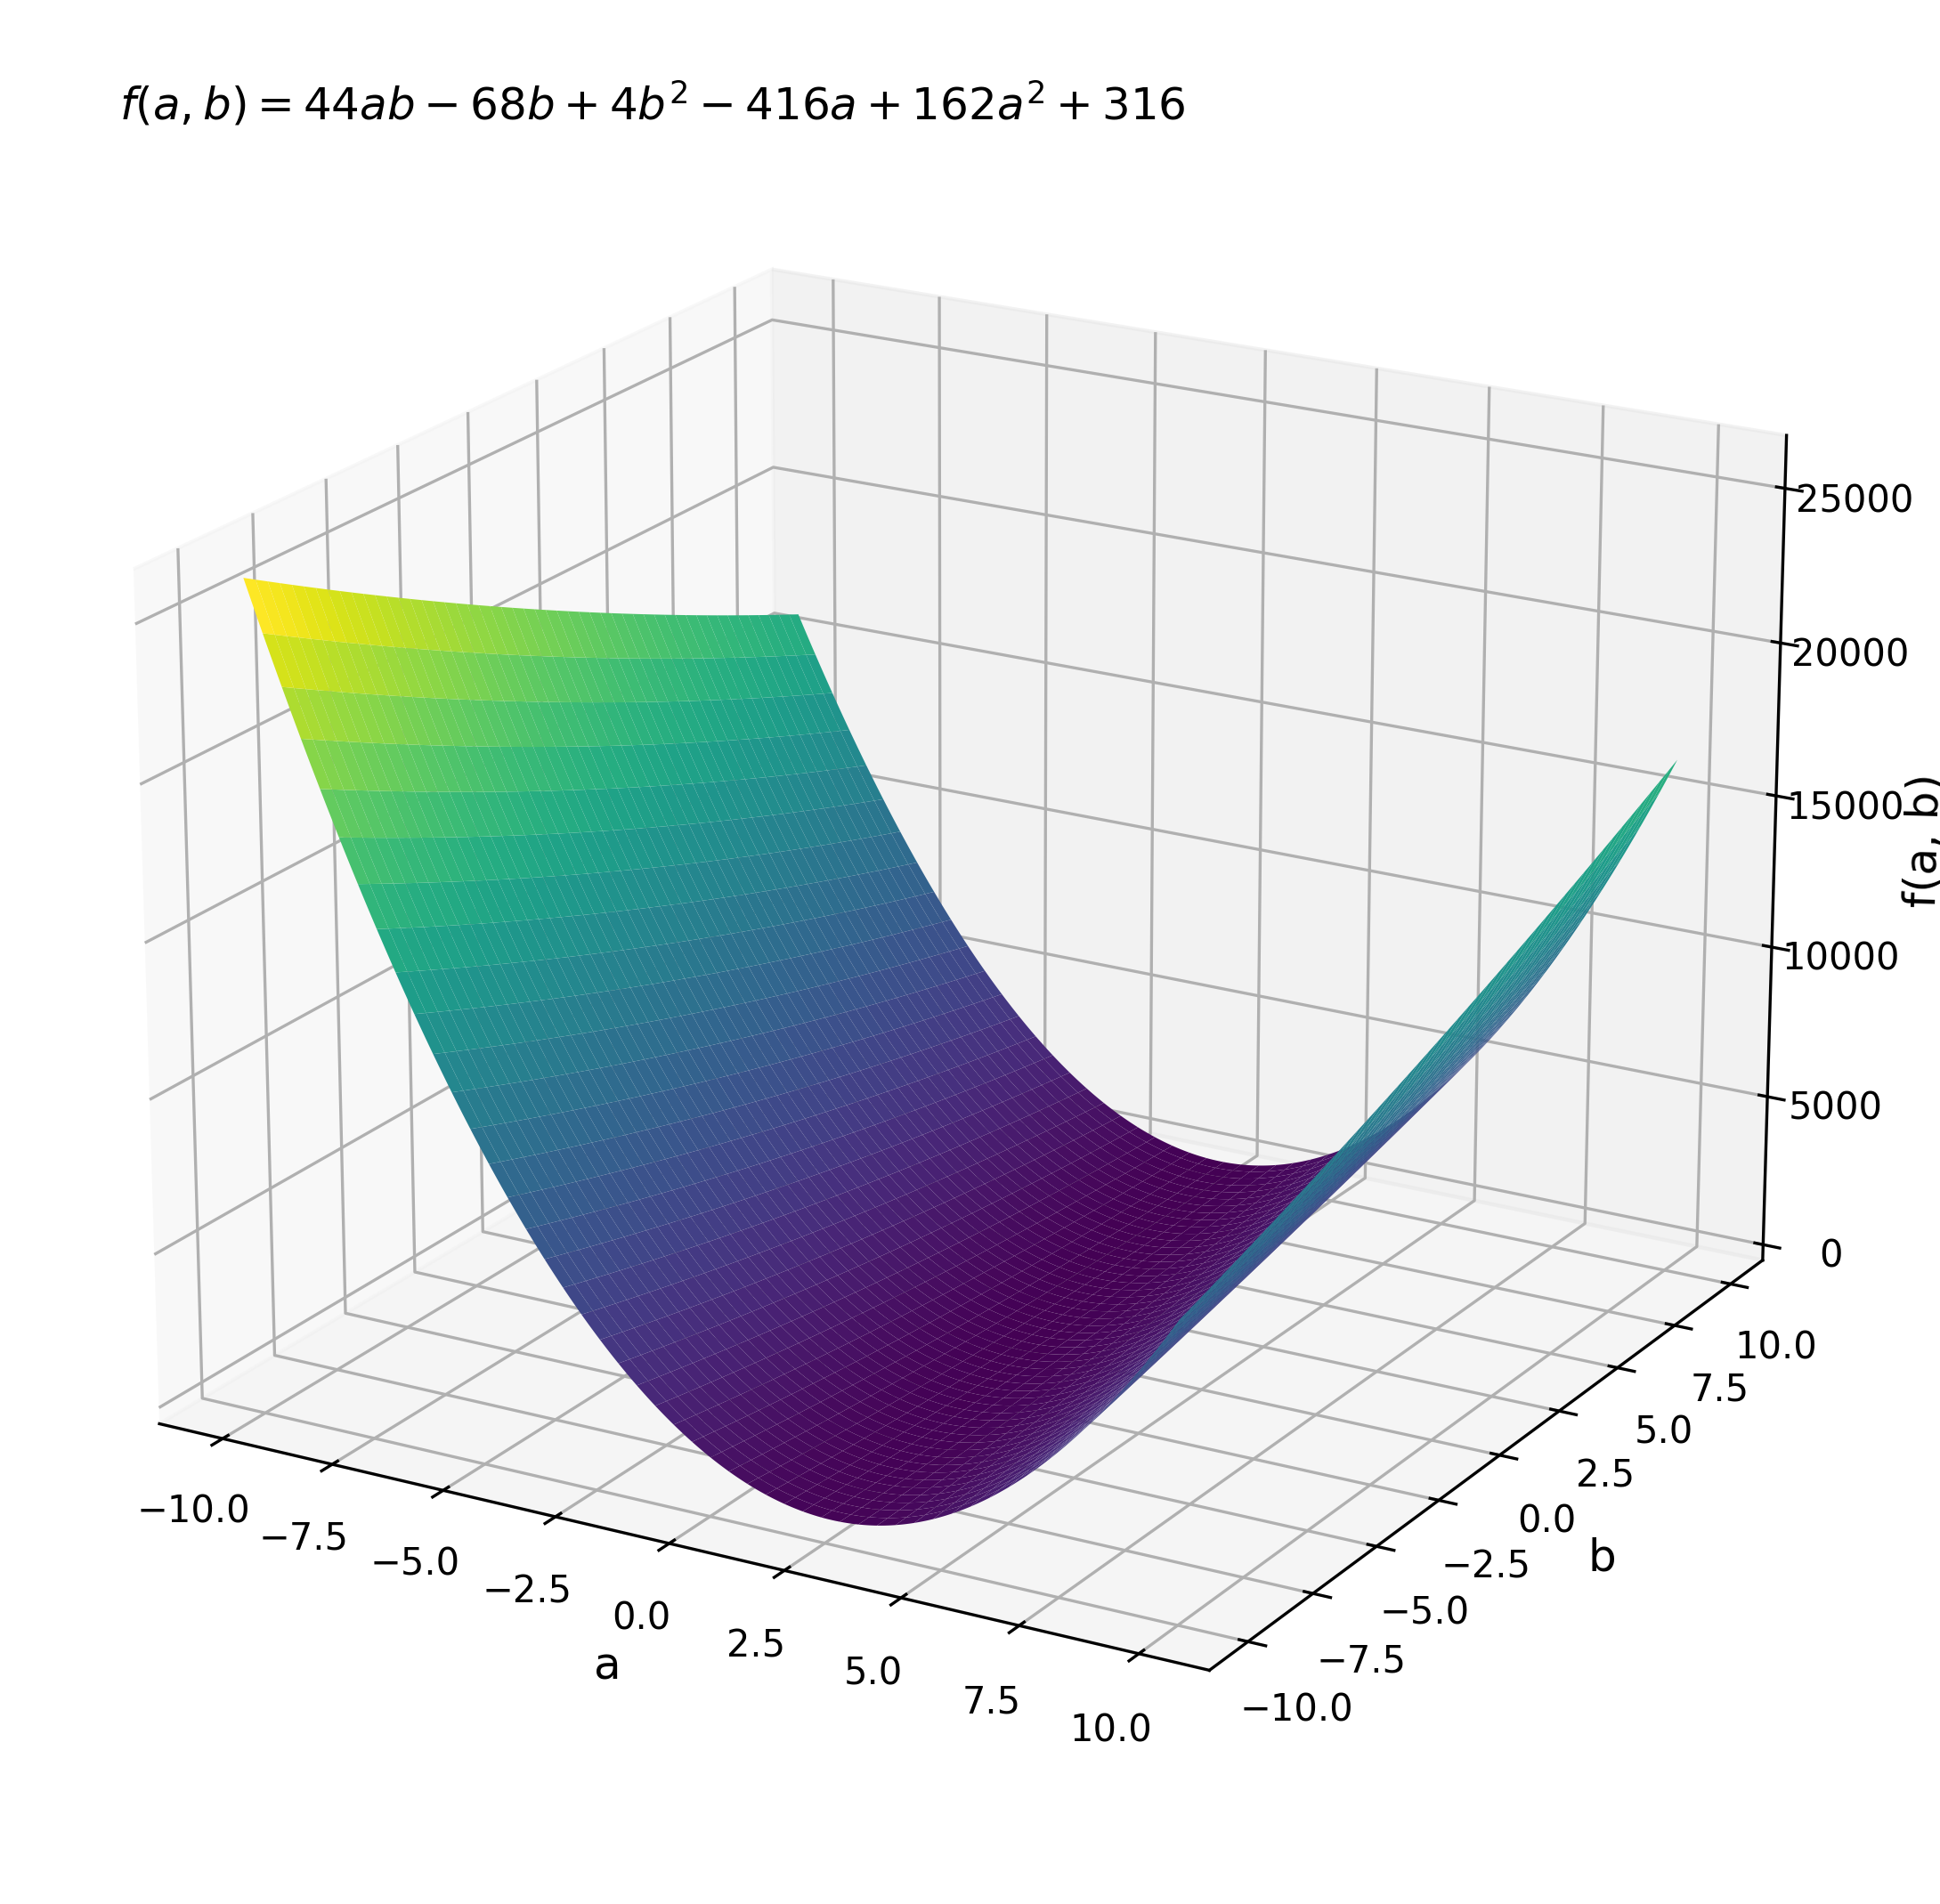
\includegraphics[width=0.5\textwidth]{figures/3dGraf.png}
    \caption{Grafisk afblidning af funktionen $f(a,b)$}
    \label{fig:grafiskAfbildningAfFunktionAfToVariable}
\end{figure}  
For at finde den funktion der passer bedst til datasættet, skal der findes det sted hvor funktionen $f(a,b)$ har et minimumspunkt (Se evt figur \ref{fig:grafiskAfbildningAfFunktionAfToVariable}) Dette gøres ved at tage partielt afledede af funktionen $f(a,b)$ med hensyn til $a$ og $b$. De differentialkvotienter der kommer ud af dette sættes til 0. 
\begin{equation*}
    \frac{\partial f(a,b)}{\partial a} = 44b + 324a - 416
\end{equation*}
\begin{equation*}
    \frac{\partial f(a,b)}{\partial b} = 8b + 44a - 68
\end{equation*}
Disse to difransialkvotienter sættes nu til 0. Dette giver følgende ligningsystem:
\begin{equation*}
    44b + 324a - 416 = 0
\end{equation*}
\begin{equation*}
    8b + 44a - 68 = 0
\end{equation*}
Dette ligningsystem kan nu løses med hensyn til $a$ og $b$. Dette giver følgende resultat:
\begin{equation*}
    a = 0,5122 
\end{equation*}
\begin{equation*}
    b = 5,68293
\end{equation*}
Resultatet af beregningerne af dette datasæt viser at denne metode godt, kan anvendes til at finde en linje der passer bedst til et datasæt. Det kan være svært at konkludere præcist hvor god den er, men resultatet er sat op mod GeoGebra og her stemmer resultaterne overens helt ned til 5 decimal.
% Synes stadig ikke helt at jeg er i mål med denne del. 

\section{Implementering af Mindste Kvadraters Metode}
Matematik og programmering hænger på mange måder naturligt godt sammen. Matematik bruges til at beskrive og forklare komplekse problemstillinger, mens programmering gør det muligt at omsætte disse problemstillinger til konkrete løsninger. Med programmering følger også en række praktiske fordele, som kan gøre selv de sværeste håndberegninger på sekunder. Dette gælder især, når man arbejder med store datasæt. Programmering giver os værktøjerne til at bearbejde data hurtigt og præcist, hvilket er noget, mennesker aldrig ville kunne gøre manuelt lige så hurtigt. \cite{codeWithC} Forestil dig for eksempel, at du har ti tusinde datapunkter fra en virksomheds salgsdata. At finde et mønster manuelt ville være en næsten umulig opgave. Her kommer computeren og programmeringen ind i billedet. Ved hjælp af simple algoritmer og lidt programmeringserfaring kan man omsætte dataene til resultater på få sekunder. Det samme gælder, når der arbejdes med Mindste Kvadraters Metode. Hvor det manuelt ville kræve mange trin og lang tid at finde den bedst passende linje, kan en computer beregne dette på ingen tid. Se bare hvor mange skridt der er blevet taget i afsnit \ref{sec:udregning} for at finde den bedst mulige linje, tænk på hvor lang tid det ville tage hvis der var mere end fire punkter. 

% Kig det her afsnit igennem
% Programmering er ikke bare hurtigere; det åbner også op for at eksperimentere og tilpasse løsninger. Har man for eksempel data, hvor nogle observationer afviger markant fra de andre, kan man justere modellen eller filtrere data for at få en bedre beskrivelse. Med Mindste Kvadraters Metode kan man også hurtigt teste, hvordan små ændringer i datasættet påvirker resultatet, og dermed finde den model, der passer bedst. Denne fleksibilitet er afgørende, især når data ikke altid opfører sig, som man forventer. En anden fordel ved at kombinere matematik og programmering er muligheden for visualisering. Når en model er blevet beregnet, kan man hurtigt lave grafer, der viser, hvordan modellen passer til data. For eksempel kan man plotte en lineær regression sammen med de oprindelige datapunkter for at få et visuelt overblik over, hvordan sammenhængen ser ud. Det gør resultaterne nemmere at forstå og formidle, og det kan give nye indsigter, som man måske ikke ville opdage alene gennem beregninger. Det er netop i kombinationen af matematik og programmering, at den virkelige styrke ligger. Matematikken giver præcision og struktur, mens programmeringen giver hastighed, fleksibilitet og mulighed for at arbejde med data i stor skala. Dette gør ikke bare processen hurtigere, men det gør det også muligt at håndtere komplekse problemstillinger, som tidligere ville have været uden for rækkevidde. Når man arbejder med metoder som Mindste Kvadraters Metode, bliver denne kombination særlig tydelig. Det er her, de abstrakte modeller møder den praktiske virkelighed, og resultaterne bliver noget, man faktisk kan bruge.
% Anvend pseudokode til at vise hvordan Mindste Kvadraters Metode kan implementeres


\subsection{Program Design}
% Forklar hvilke overvejelser der er gjort i forhold til program design, sprogvalg, biblioteker, etc. Teorisk baggrund!!!

\subsection{Program redegørsel}
% Redegør for programmet og dets funktioner (Husk at inkludere kodeeksempler)

\section{Fordele og Begrænsninger}
%Her analyseres metoden på et bredere niveau ved at vurdere dens styrker og svagheder i en programmeringssammenhæng.

\section{Diskussion af Kodningsmetoder}
% While loops, for loops, rekursive funktioner, ect.

\section{Konklusion}

\section{Perspektivering}
